\chapter{Probleembeschrijving}
\label{chap:Probleembeschrijving}

Dit hoofdstuk beschrijft het probleem van automatische afbeeldingsbeschrijving. Een eerste sectie gaat over het concrete vraagstuk en hoe het gesitueerd is binnen de computerwetenschappen. Een tweede sectie beschrijft de datasets die algemeen gebruikt worden voor het trainen en evalueren van systemen.

\section{Omschrijving en situering}
\label{sec:Omschrijving en situering}

\section{Datasets}
\label{sec:Datasets}
Deze sectie beschrijft de drie meest gebruikte datasets voor training en evaluatie van modellen voor afbeeldingsbeschrijving: Flickr8k, Flickr30k en MS COCO.

\paragraph{Flickr8k}
\label{par:Flickr8k}
De Flickr8k dataset, zoals voorgesteld in \todo{ref} bevat 8,092 foto's vanop \texttt{flickr.com}. De focus doorheen de afbeeldingen ligt op mensen en dieren (vooral honden) die een actie uitvoeren. De foto's zijn manueel geselecteerd om de grootst mogelijke vari\"eteit te garanderen.

De bijhorende beschrijvingen zijn manueel opgesteld door mensen met Engels als moedertaal. Een voorafgaande test van de personen die de zinnen schrijven moet de correctheid van de beschrijvingen garanderen. Eenzelfde afbeelding kan tot verschillende beschrijvingen leiden: sommige mensen focussen op de actie, anderen leggen de nadruk op de persoon die de actie uitvoert, \ldots De zinnen \texttt{A man is skiing down a hill} en \texttt{A man is going down a hill on his skis} beschrijven dezelfde foto, maar doen dit op een verschillende manier. Om deze rijkdom in taal te kunnen weergeven zijn er meerdere zinnen per afbeelding opgenomen in de dataset.

De dataset is verdeeld in drie delen, voor training, validatie en testing. De validatie- en testset bevatten elk 1000 foto's, de trainingsset bevat de overige 6092.


\paragraph{Flickr30k}
\label{par:Flickr30k}
Deze dataset \todo{referenceeeeeee} is een uitbreiding van Flickr8k. In totaal zijn er 31,783 foto's, met elk 5 beschrijvingen. Het proces dat gebruikt is om de dataset op te stellen is hetzelfde als bij Flickr8k \todo{nog is ref? of nie?} en ook hier bestaan de test- en validatieset uit 1000 foto's, met de resterende 29,783 in de trainingsset.


\paragraph{MS COCO}
\label{par:MS COCO}
De Microsoft Common Objects in COntext dataset(MS COCO) \todo{reference} staat los van de Flickr datasets en probeert een ander type van afbeelding te brengen. Ze bevat meer dan 330,000 afbeeldingen die elk vijf beschrijvingen hebben.

MS COCO probeert meer te bieden dan ``standaard'' foto's. De auteurs maken een onderscheid tussen afbeeldingen van iconische objecten en iconische sc\`enes, en non-iconische afbeeldingen. Iconische afbeeldingen vormen typisch de eerste zoekresultaten bij een Google Image Search, maar ze bevatten te weinig informatie. Bijgevolg leiden ze ook tot minder interessante beschrijvingen. Non-iconische afbeeldingen brengen algemeen gezien een compositie van verschillende objecten en personen, gefotografeerd vanuit een niet-canonische hoek. Figuur \ref{fig:cocotypes} toont duidelijk het verschil tussen iconische en non-iconische afbeeldingen.

\begin{figure}[tb]
    \centering
    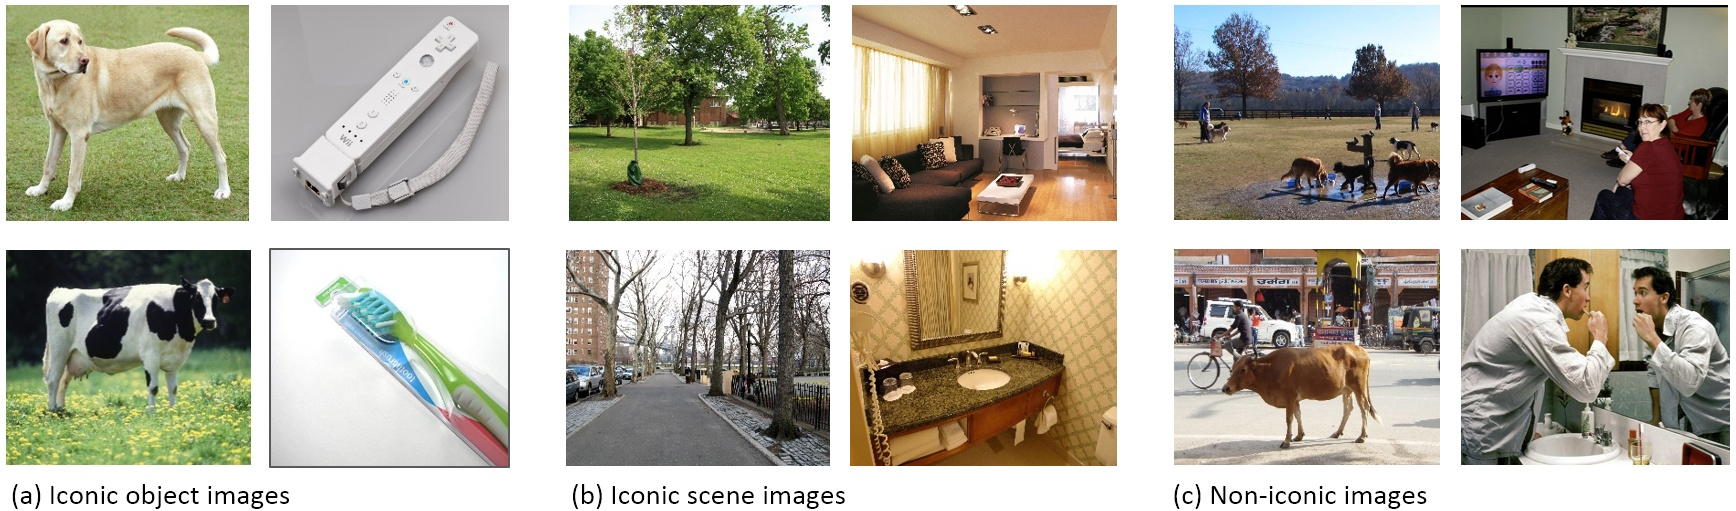
\includegraphics[width=\linewidth]{Images/iconic.jpg}
    \caption{Verschil tussen iconische en non-iconische afbeeldingen}
    \label{fig:cocotypes}
\end{figure}

Een ander belangrijk deel van de dataset zijn annotaties. Oudere datasets legden de focus op classificatie, bounding boxes en segmentatie, terwijl MS COCO probeert om elk belangrijk object op de foto te annoteren. 

Het genereren van de beschrijvingen bij de foto's gebeurt met AMT workers, net zoals bij de Flickr datasets. Uitgebreide instructies voor de workers garanderen dat elk belangrijk deel van de afbeelding voorkomt in de beschrijving. \todo{reference naar coco generation paper}
